\pdfminorversion=4
\documentclass[aspectratio=1610,t,10pt]{beamer}

\usepackage[utf8]{inputenc}

\usepackage{standalone}
\usepackage{multimedia}
\usepackage[font=footnotesize]{subcaption}
\usepackage{tikzscale}

\usepackage{mathptmx}
\usepackage{tikz}
\usepackage{pgfplots}
\pgfplotsset{compat=newest}
\usetikzlibrary{arrows}
\usetikzlibrary{shapes}
\usetikzlibrary{positioning}
\usetikzlibrary{fit}
\providecommand{\includetikz}[2][1]{\tikzset{every picture/.style={scale=#1}}\includestandalone{#2}}

\title{Dislocation Dynamics Simulation}
\subtitle{Large scale simulations with Numodis}
\date{May 12, 2018}
\author[Arnaud Durocher]{Arnaud \textsc{Durocher}}
\institute[MdlS]{}
\titlegraphic{\includegraphics[width=7cm]{img/1st_page.png}}

\usepackage{theme/beamerthemecea}

\newlength{\freeheight}
\setlength{\freeheight}{0.83\textheight}

\begin{document}

\captionsetup{size=footnotesize,justification=centering,skip=1pt}

\begin{frame}[plain]
    \titlepage
\end{frame}

\begin{frame}
	\frametitle{Table of Contents}
	\framesubtitle{}
	\begin{columns}[t]
		\begin{column}{\textwidth}
			\tableofcontents
		\end{column}
	\end{columns}
\end{frame}

\section{Context}

\subsection{Introduction}

\begin{frame}
    \frametitle{Introduction}
    \framesubtitle{Dislocation Dynamics for Nuclear Materials}
    \begin{columns}[c]
	    \begin{column}{.48\textwidth}
	        
	        	\begin{block}{Studied Effects}
	        		\begin{itemize}
	        			\item Material ageing under irradiation
	        			\item Hardening, embrittlement, creep, ...
	        		\end{itemize}
	        	\end{block}
	       
	        \begin{figure}
	            \centering
	            \begin{subfigure}[t]{0.38\textwidth}
	                \centering
	                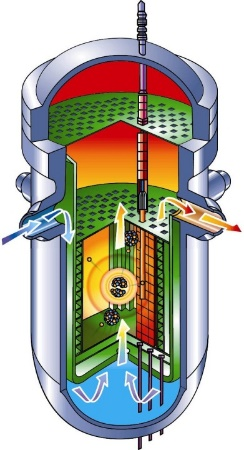
\includegraphics[height=0.5\freeheight, keepaspectratio]{img/vessel}
	                \caption{Vessel (Steel) }
	            \end{subfigure}
	            \begin{subfigure}[t]{0.58\textwidth}
	                \centering
	                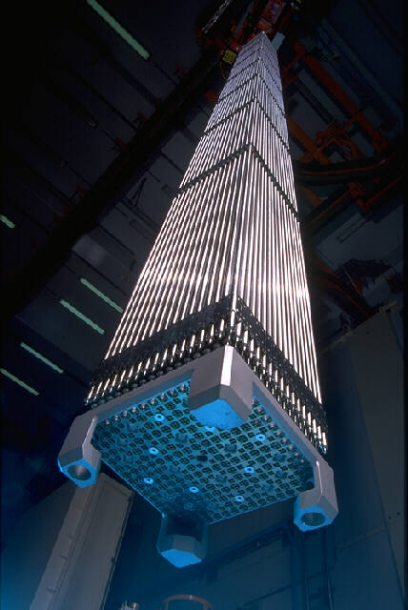
\includegraphics[height=0.5\freeheight, keepaspectratio]{img/claddings}
	                \caption{Fuel Assembly (Zirconium)}
	            \end{subfigure}
	        \end{figure}
	    \end{column}
	    \begin{column}{.48\textwidth}
		    	\centering
		    \begin{figure}
		    	\begin{subfigure}[c]{0.48\textwidth}
		    		\centering
		    		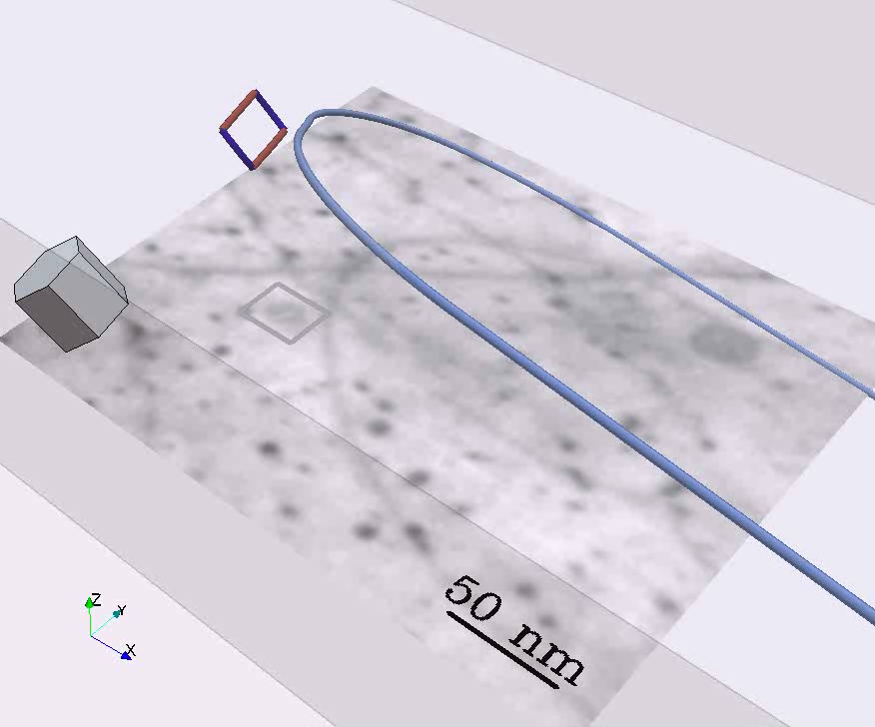
\includegraphics[width=\linewidth, keepaspectratio]{img/dd-in-situ}
		    		\caption{ Drouet et al. 2016 }
		    	\end{subfigure}
		    	\begin{subfigure}[c]{0.48\textwidth}
		    		\centering
		    		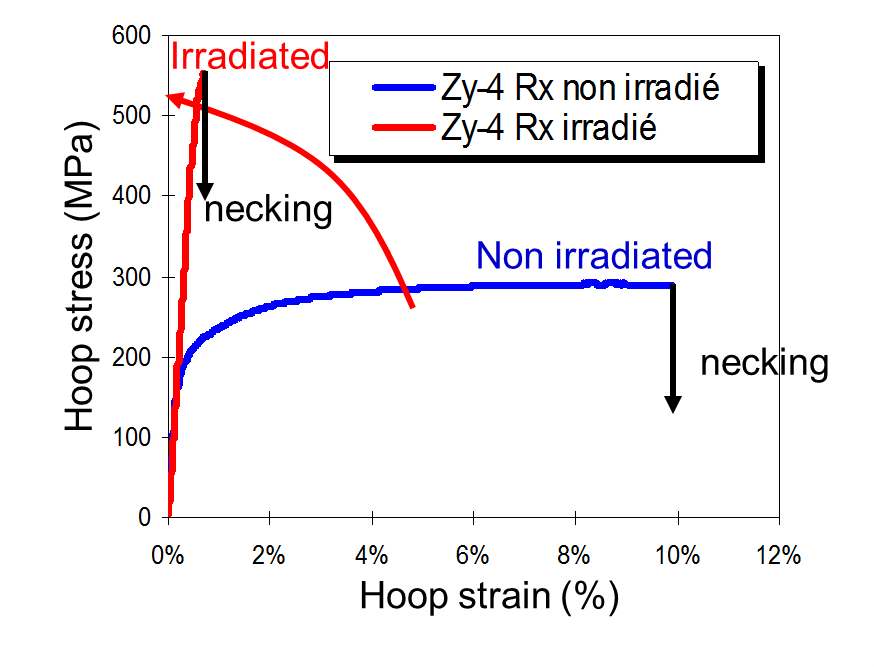
\includegraphics[width=\linewidth, keepaspectratio]{img/sigeps}
		    		\caption{ Onimus et al.}
		    	\end{subfigure}
	    	\end{figure}
		    	\begin{block}{Dislocations}
	            \begin{itemize}
	            	\item Linear defects in cristalline materials;
	            	\item Modeling plasticity in solids
	            \end{itemize}
            	 \end{block}        
	    \end{column}
    \end{columns}
\end{frame}

%\begin{frame}
%\frametitle{Introduction}
%\framesubtitle{Multi-scale modeling of materials}

%\centering

%\includegraphics{img/multiscale_modeling/multiscale_modeling.tikz}
%\end{frame}

\begin{frame}
\frametitle{Introduction}
\framesubtitle{Visual example (Shi - 2014)}
\centering

\begin{overprint}
	\foreach \n in {1,...,4}{
		\includegraphics<\n>[width=\textwidth]{img/numo-example/numodis-\n}
	}
\end{overprint}	
\end{frame}

\begin{frame}
    \frametitle{Introduction}
    \framesubtitle{Large scale Dislocation Dynamics with Numodis}
    \begin{columns}[c]
    \begin{column}{.44\textwidth}
        \begin{block}{Numodis}
            \begin{itemize}
                \item Mono-CPU computations
                \item Up to 10 000 dislocations segments
            \end{itemize}
       	\end{block}
	     \begin{figure}
	        	\centering
	        	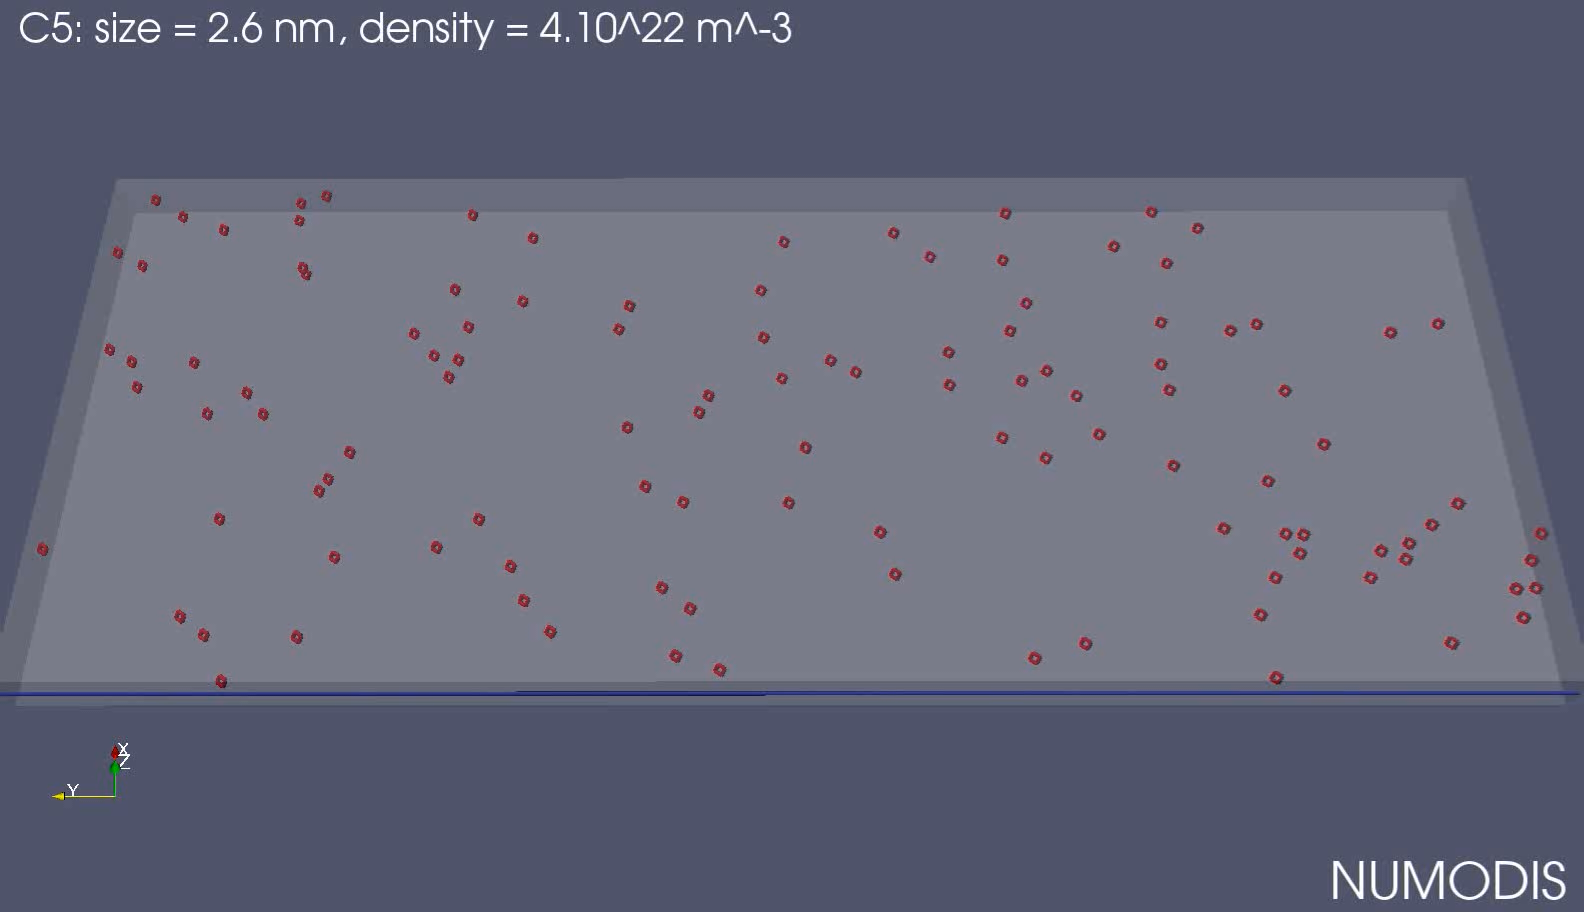
\includegraphics[height=0.5\freeheight]{img/numo-example/numodis-1}
	     \end{figure}        
    \end{column}
	\begin{column}{.05\textwidth}
		\centering
		\textbf{\Large$\Rightarrow$}        
	\end{column}
    \begin{column}{.44\textwidth}
    	\begin{block}{Parallel Numodis}
    		\begin{itemize}
    			\item Parallel and distributed architectures
    			\item Up to 1 000 000 dislocations segments
    		\end{itemize}
    	\end{block}
    	\begin{figure}
    		\centering
    		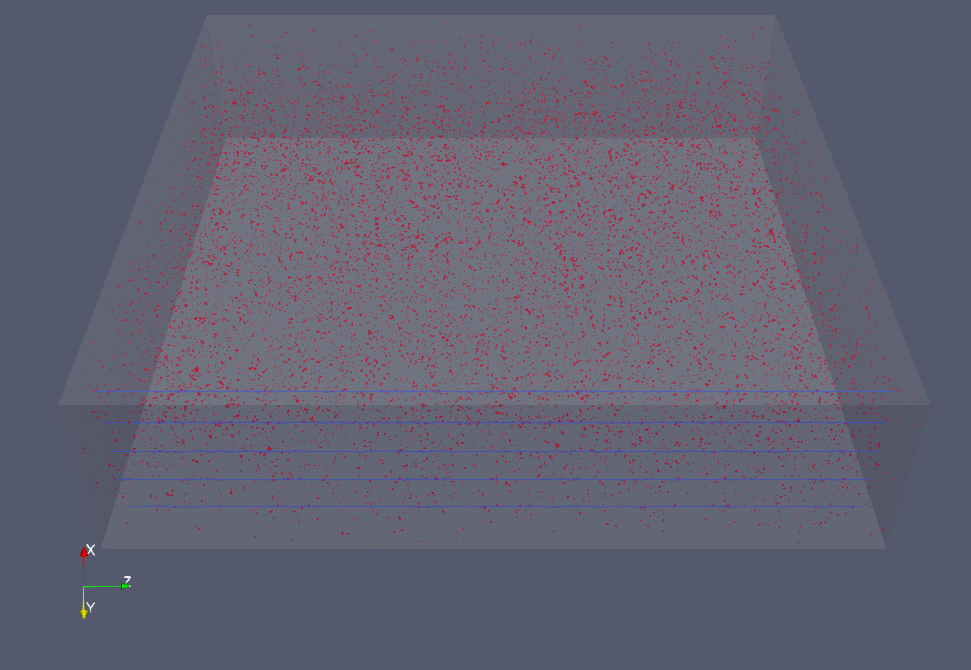
\includegraphics[height=0.5\freeheight]{img/basalglide_big}
    	\end{figure}        
    \end{column}
    \end{columns}
    \vfill
    \centering
    
    \textbf{$\Rightarrow$ Simulate a dislocation mesh dense enough to reliably modelise a grain.}
\end{frame}


\subsection{Discrete Dislocation Dynamics Simulation}

\subsubsection{Step-by-Step Algorithm}

\begin{frame}
	\frametitle{Discrete Dislocation Dynamics Simulation}
	\framesubtitle{Step-by-Step Algorithm}
	
	\begin{columns}[c]
		\begin{column}{.45\textwidth}
			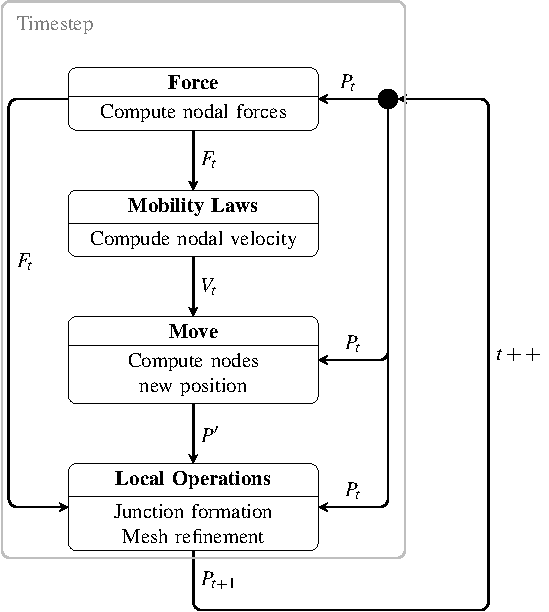
\includegraphics[height=\freeheight]{img/simulation-steps.pdf}
		\end{column}
		\begin{column}{.45\textwidth}
			\centering
			\begin{overprint}
				\foreach \n in {1,...,5}{
					\includegraphics<\n>[height=\freeheight, width=\textwidth, keepaspectratio]{img/ddd-algo/ddd_algo-\n.pdf}
				}
			\end{overprint}
		\end{column}
	\end{columns}
	
\end{frame}

\begin{frame}
	\frametitle{Discrete Dislocation Dynamics Simulation}
	\framesubtitle{Hotspots}
	
	\begin{columns}[c]
		\begin{column}{.45\textwidth}
			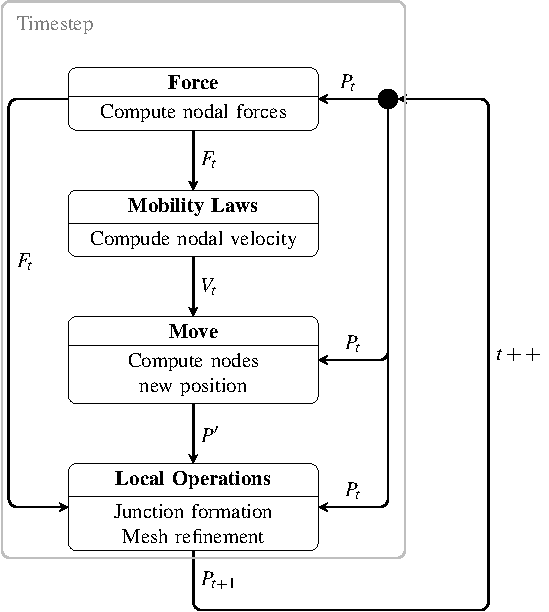
\includegraphics[height=\freeheight]{img/simulation-steps.pdf}
		\end{column}
		\begin{column}{.45\textwidth}
			\centering
			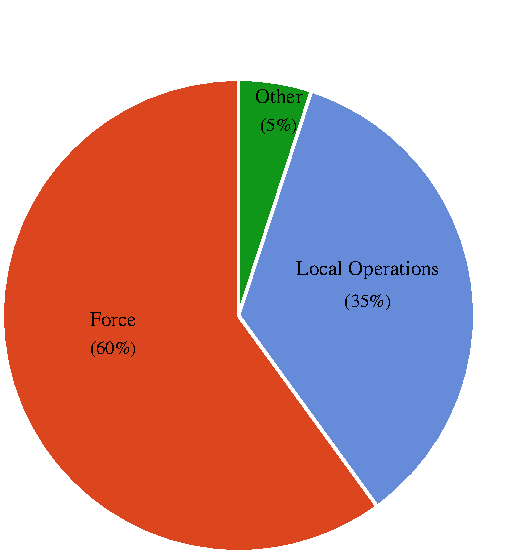
\includegraphics[width=0.8\textwidth]{img/hotspots.pdf}
		\end{column}
	\end{columns}
	
\end{frame}

\begin{frame}
    \frametitle{Discrete Dislocation Dynamics Simulation}
    \framesubtitle{Fast Multipole Method}
    \begin{columns}[c]
    \begin{column}{.48\textwidth}
        \centering
        
        \vspace{1em}
        
        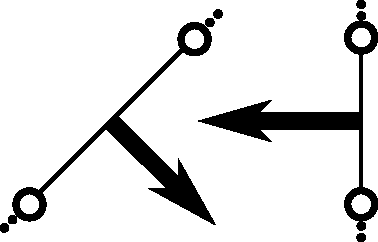
\includegraphics[height=0.3\freeheight, keepaspectratio]{img/elastic_force.pdf}
        
        {\small Peach-Koehler Force between dislocation segments}
        
        \vspace{1em}
        
        \begin{block}{Fast Multipole Method}
            \begin{itemize}
                \item Far-field approximation
                \item Hierarchical Domain Decomposition
                \item ScalFMM (inria Hiepacs)
            \end{itemize}
            \textbf{ $\sim$ N complexity}
        \end{block}
    \end{column}
    \begin{column}{.48\textwidth}
        \begin{block}{Segment Elastic Interaction}
            \begin{itemize}
                \item Interact with each other
            \end{itemize}
            \textbf{ N$^2$ complexity}
        \end{block}
        \vspace{2em}
        \centering
        
\includegraphics[width=0.7\textwidth, keepaspectratio]{img/scalfmm}   
             
        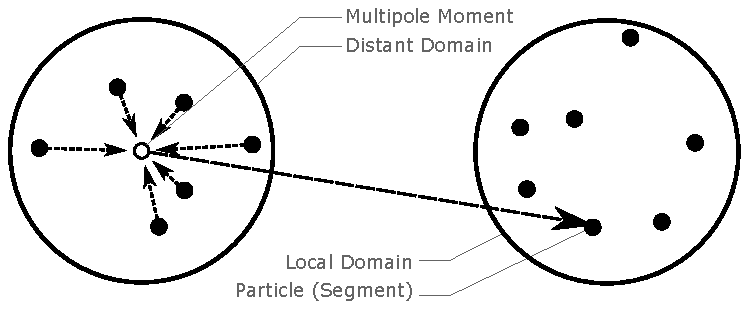
\includegraphics[width=\textwidth, keepaspectratio]{img/far_field.pdf}
    \end{column}
    \end{columns}
\end{frame}

\section{Contributions}
\subsection*{}
\begin{frame}

\begin{minipage}[c][\freeheight]{\textwidth}
	{\Huge \bf Contributions}
\end{minipage}

\begin{tikzpicture}[remember picture,overlay,every node/.style={inner sep=0,outer sep=0}]
\node[anchor=north east, xshift=0.5cm] at (current page.north east) {
\includegraphics[height=\the\paperheight]{theme/graphics/cea_square.png}};
\end{tikzpicture}
\end{frame}

\subsection{Distributed datastructure for Dislocation Dynamics}

\subsubsection{Designing a datastructure for Dislocation Dynamics}

\begin{frame}
	\frametitle{Datastructure for Dislocation Dynamics}
    \framesubtitle{Designing the datastructure}
    \begin{columns}[c]
    	\begin{column}{.48\textwidth}
    		\centering      
    		\begin{figure}		  		
    		\includetikz[0.4]{img/dislocation-discrete}
    		\end{figure}    	\end{column}
	    \begin{column}{.48\textwidth}
	    	\begin{block}{Node and segment data}				
	    		\begin{columns}[t]
	    			\begin{column}{0.35\columnwidth}
	    				Nodes :
	    				\begin{itemize}
	    					\item Position
	    					\item Velocity
	    					\item Force 
   	    				\end{itemize}
	    			\end{column}
	    			\begin{column}{0.55\columnwidth}
	    				Segments :
	    				\begin{itemize}
	    					\item End nodes forces
	    					\item Physical properties
	    					\begin{itemize}
	    						\item Burgers vector
	    						\item Glide plane
	    					\end{itemize}
	    				\end{itemize}
	    			\end{column}
	    		\end{columns}
	    	\end{block}
	    \end{column}
    \end{columns}
	\begin{block}{Operations on data}
		\begin{columns}[t]
			\begin{column}{0.45\columnwidth}
				Topological operations :
				\begin{itemize}
					\item Add/remove nodes
					\item Add/remove segments
				\end{itemize}
				$\rightarrow$\textit{Dynamic mesh}
			\end{column}
			\begin{column}{0.45\columnwidth}
				Iterate over nodes and segments:
				\begin{itemize}
					\item Nodes with connected segments
					\item Segments with connected nodes
				\end{itemize}
				$\rightarrow$\textit{Irregular access}
			\end{column}
		\end{columns}
	\end{block}
\end{frame}

\subsubsection{Datastructure for distributed memory clusters}

\begin{frame}
\frametitle{Datastructure for Dislocation Dynamics}
\framesubtitle{Distributed data with MPI}
\begin{columns}[c]
	\begin{column}{.48\textwidth}
		\centering   		  		
		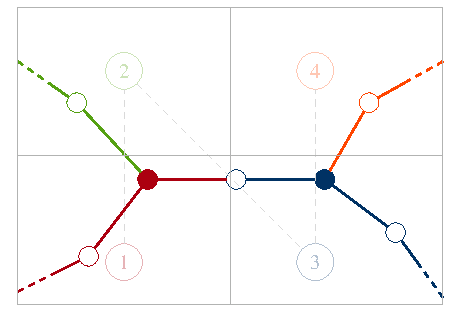
\includegraphics[width=\textwidth]{img/dislocations-distribuees}
	\end{column}
	\begin{column}{.48\textwidth}
		\begin{block}{Distributed data (MPI)}
			\begin{itemize}
				\item Too big to fit in 1 computer
				\item Distributed supercomputers
			\end{itemize}
		\end{block}
		\begin{block}{Challenges}
			\begin{itemize}
				\item Keep data coherency
				\item Access remote data
			\end{itemize}
		\end{block}
	\end{column}
\end{columns}
\begin{block}{$\Rightarrow$ Distributed Abstract Datatype}
	\begin{columns}[c]
		\begin{column}{.48\textwidth}
			\begin{itemize}
				\item Safe mesh modification
				\item Safe access to remote data
			\end{itemize}
		\end{column}
		\begin{column}{.48\textwidth}
			\begin{itemize}
				\item Easier to use to write algorithms
				\item Easier to change implementation
			\end{itemize}
		\end{column}
	\end{columns}
\end{block}
\end{frame}



\subsection{Collision algorithm for junction formation}

\begin{frame}
\frametitle{Collision algorithm}
\framesubtitle{Mechanisms of junction formation}
\begin{columns}[c]
	\begin{column}{.48\textwidth}
		\begin{block}{Dislocation Junctions}
			\begin{itemize}
				\item Merging of dislocations at collision;
				\item Important role in material behavior \\ (strain and radiation hardening)
			\end{itemize}
		\end{block}
		\vspace{1em}
		\centering
		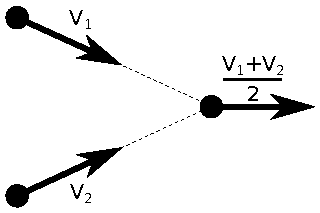
\includegraphics[height=0.25\freeheight]{img/collision_topo_poinpoint}
		
		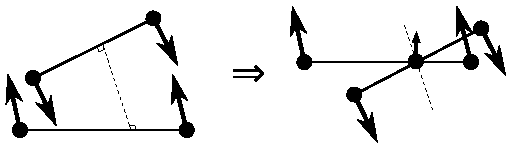
\includegraphics[height=0.25\freeheight]{img/collision_topo_segseg}
	\end{column}
	\begin{column}{.48\textwidth}
		\begin{figure}
			\centering
			\caption*{Dislocation multi-junctions and strain hardening \\ (Bulatov et al. - nature 2006)}
			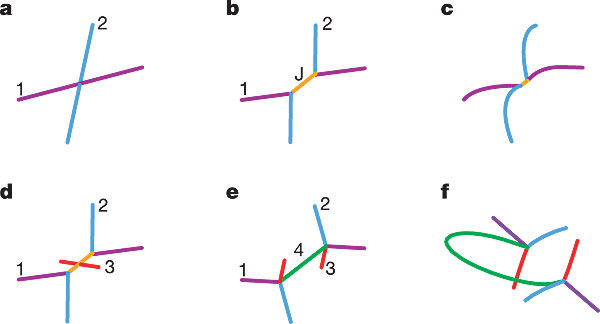
\includegraphics[width=0.7\textwidth]{img/junction_nature}
		\end{figure}
		\begin{block}{Simulate junction formation}
			\begin{itemize}
				\item \textbf{Collision detection} (N body) \\ {\footnotesize$\rightarrow N^2$ complexity}
				\item Handle dislocation merging.
			\end{itemize}
		\end{block}		
	\end{column}
\end{columns}
\end{frame}

\subsubsection{Fast collision detection}

\begin{frame}
\frametitle{Collision algorithm}
\framesubtitle{Fast collision detection}
\vspace{1em}
\begin{columns}[c]
	\begin{column}{.48\textwidth}
		\begin{block}{Uniform grid space partitioning}
			\begin{itemize}
				\item Only test collision on nearby boxes;
				\item Determined the minimum box size \\ \textit{~\footnotesize Depends on object size and velocity}
			\end{itemize}
			\centering
			\textbf{Complexity N$^2$ to $\sim$ N}								
		\end{block}
	\end{column}
	\begin{column}{.48\textwidth}
		\centering
		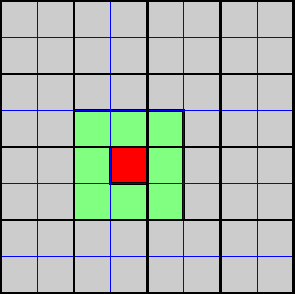
\includegraphics[width=0.4\textwidth]{img/uniform_grid}
		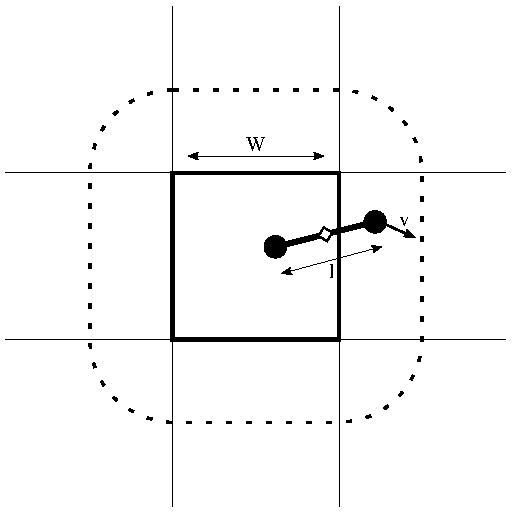
\includegraphics[width=0.4\textwidth]{img/minimum_box_size}		
	\end{column}
\end{columns}
\vspace{1ex}
\begin{columns}[c]
	\begin{column}{.48\textwidth}
		\centering
		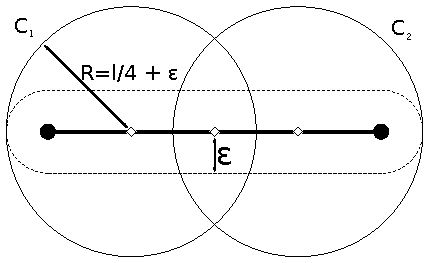
\includegraphics[width=0.8\textwidth]{img/bounding_spheres}
	\end{column}
	\begin{column}{.48\textwidth}
		\begin{block}{Bounding spheres}
			\begin{itemize}
				\item Segments simplified by 2 spheres;
				\item Sphere/Sphere collision faster to detect;
				\item Smaller objects $=$ Smaller box size.					
			\end{itemize}				
		\end{block}
	\end{column}
\end{columns}
\end{frame}

\subsubsection{Accurate collision handling}

\begin{frame}
\frametitle{Collision algorithm}
\framesubtitle{Accurate collision handling}
\begin{columns}[c]
	\begin{column}{.48\textwidth}
		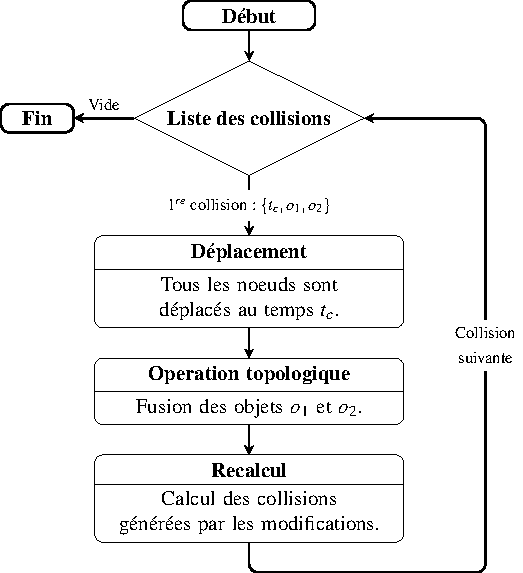
\includegraphics[height=\freeheight]{img/algo-collision}
	\end{column}
	\begin{column}{.48\textwidth}
		\begin{block}{New topological operations}
			\begin{itemize}
				\item Nodes/segments fusion on collision
				\item Using new datastructure
			\end{itemize}
		\end{block}
		\begin{block}{Collision recomputation}
			\begin{itemize}
				\item Mesh modifications can generate more collisions
				\item One object can collide into multiple objects in one timestep
			\end{itemize}
		\end{block}
		\textbf{$\Rightarrow$ More reliable collision handling}
		
	\end{column}
\end{columns}
\end{frame}


\section{Results}
\begin{frame}

\begin{minipage}[c][\freeheight]{\textwidth}
	{\Huge \bf Results}
\end{minipage}

\begin{tikzpicture}[remember picture,overlay,every node/.style={inner sep=0,outer sep=0}]
\node[anchor=north east, xshift=0.5cm] at (current page.north east) {
\includegraphics[height=\the\paperheight]{theme/graphics/cea_square.png}};
\end{tikzpicture}
\end{frame}

\subsection{Accuracy}

\subsubsection{Validation of collision algorithm}

\begin{frame}
\frametitle{Accuracy}
\framesubtitle{Validation of collision algorithm}
\vspace*{-1em}
\begin{columns}[t]
	\begin{column}{.48\textwidth}
		\begin{block}{More reliable collision handling}
			\begin{itemize}
				\item Complex geometry;
				\item Multiple collisions.
			\end{itemize}
			\centering
			\textbf{Detect collisions missed before}
		\end{block}
		\centering
		\begin{minipage}{0.30\linewidth}
			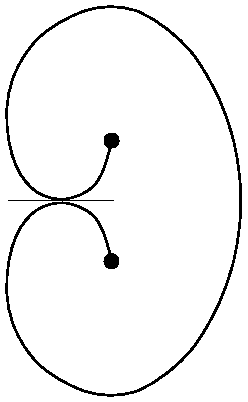
\includegraphics[width=\linewidth]{img/frankread}
		\end{minipage}~~~~%
		\begin{minipage}{0.49\linewidth}
			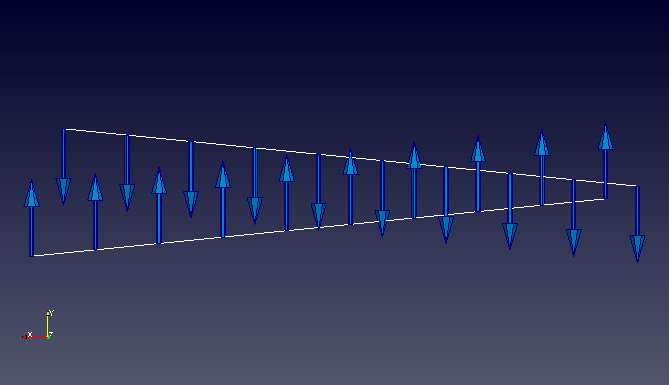
\includegraphics[width=\linewidth]{img/Initial}
			
			
			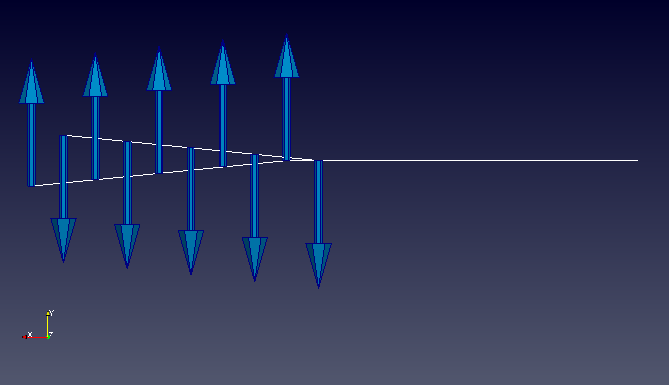
\includegraphics[width=\linewidth]{img/expected} 
		\end{minipage}			
	\end{column}
	\begin{column}{.48\textwidth}
		\begin{block}{Impact of collision recomputation}
		\centering		
		\begin{figure}
			\centering
			\begin{subfigure}[t]{0.48\textwidth}
				\centering
				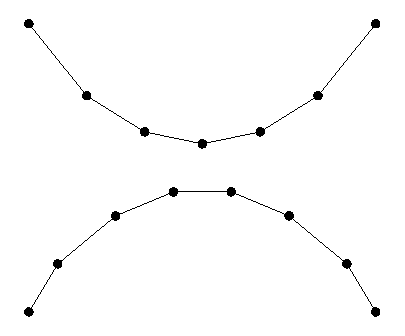
\includegraphics[width=0.8\linewidth]{img/res-collision/disloc-plot-1}
				\caption{Initial (t=0)}
			\end{subfigure}
			\begin{subfigure}[t]{0.48\textwidth}
				\centering
				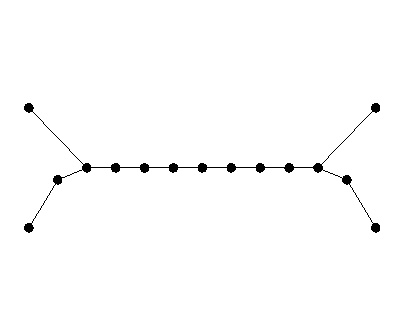
\includegraphics[width=0.8\linewidth]{img/res-collision/disloc-plot-2}
				\caption{Expected result}
			\end{subfigure}
			
			\begin{subfigure}[t]{0.48\textwidth}
				\centering
				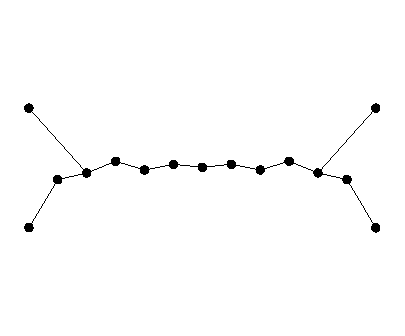
\includegraphics[width=0.8\linewidth]{img/res-collision/disloc-plot-3}
				\caption{Result with recomputation}
			\end{subfigure}
			\begin{subfigure}[t]{0.48\textwidth}
				\centering
				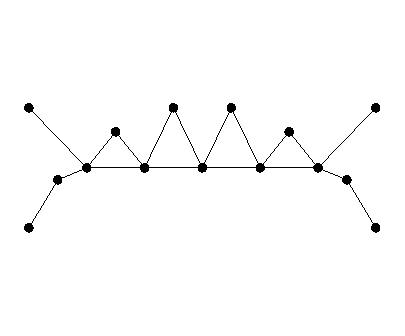
\includegraphics[width=0.8\linewidth]{img/res-collision/disloc-plot-4}
				\caption{Result without recomputation}
			\end{subfigure}
		\end{figure}
		\end{block}
	\end{column}
\end{columns}
\end{frame}

\subsubsection{Full simulation validation}

\begin{frame}
\frametitle{Accuracy}
\framesubtitle{Full simulation validation}
\centering
\begin{block}{Simulation is validated with known results from the litterature}
	\begin{figure}
		\centering
		\begin{overprint}
			\foreach \n in {1,...,5}{
				\includegraphics<\n>[height=0.7\freeheight]{img/frankread/frankread-\n.png}
			}
		\end{overprint}
		\caption{The Frank-Read source}
	\end{figure}
	\centering
\end{block}
\end{frame}

\begin{frame}
\frametitle{Accuracy}
\framesubtitle{Full simulation validation}
	\centering
	\begin{block}{Simulation is validated with known results from the litterature}
	\begin{figure}
		\begin{subfigure}{0.49\textwidth}
			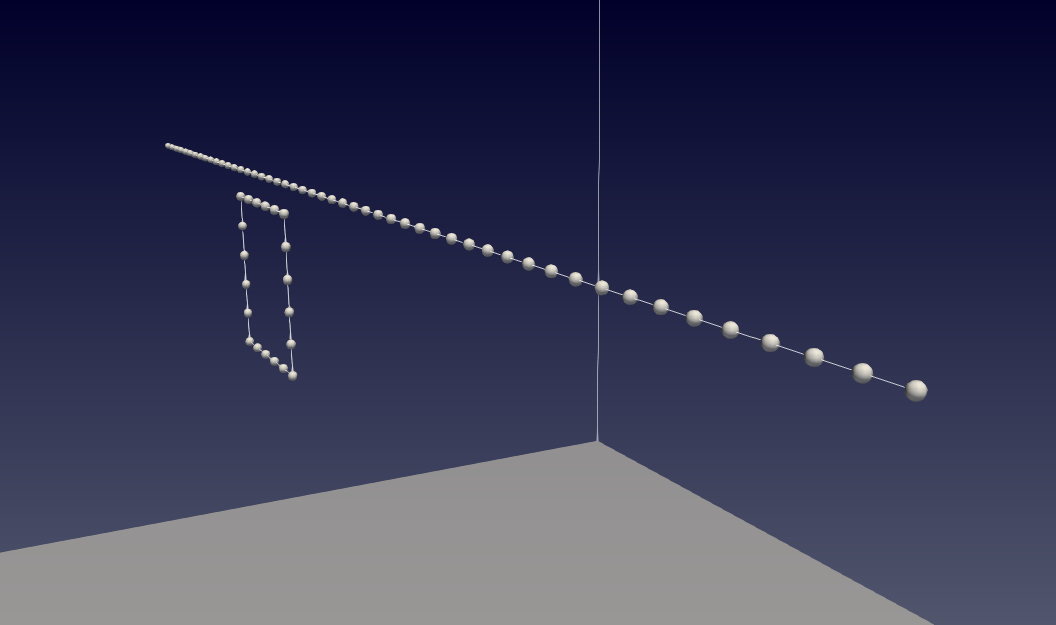
\includegraphics[width=\linewidth]{img/sb_initial.png}
			\caption{Initial situation}
		\end{subfigure}		
		\begin{subfigure}{0.49\textwidth}
			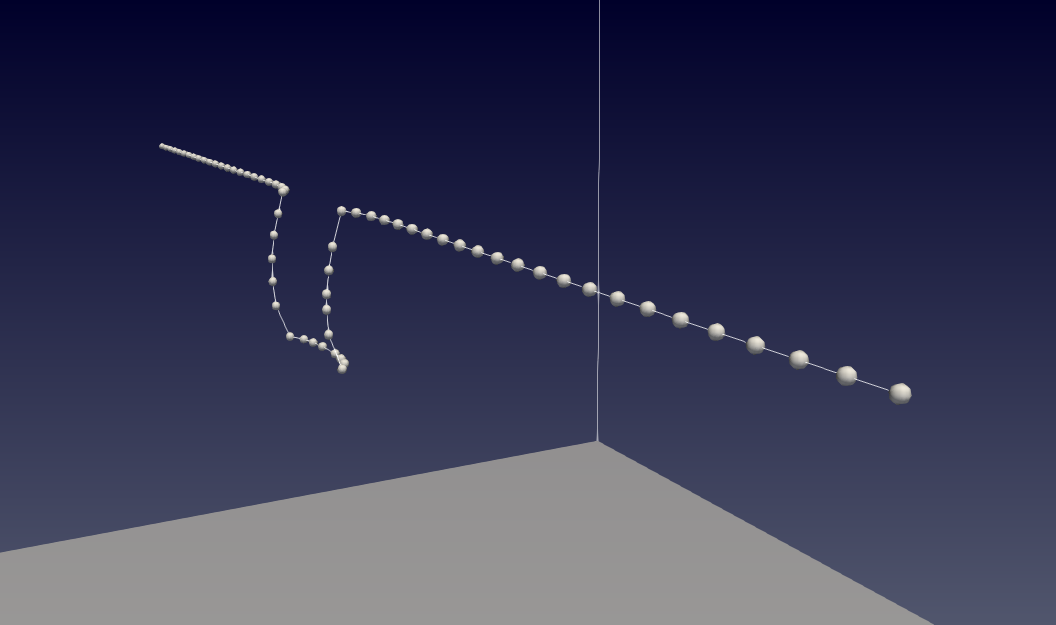
\includegraphics[width=\linewidth]{img/sb_final.png}
			\caption{Final situation}
		\end{subfigure}
	\end{figure}
	\centering
	Comparison to known Molecular Dynamics simulations \footnote{\tiny Serra \& Bacon - 2013 - "Atomic-level computer simulation of the interaction between $\frac{1}{3}\langle 1\,1\,\bar{2}\,0 \rangle\{1\,\bar{1}\,0\,0\}$ dislocations and $\frac{1}{3}\langle 1\,1\,\bar{2}\,0 \rangle$ interstitial loops in  $\alpha$-zirconium"}
	\end{block}
\end{frame}

\subsection{Performance}

\subsubsection{Large scale simulations}

\begin{frame}
\frametitle{Performance}
\framesubtitle{Large scale simulations}
\centering
\begin{overprint}
	\foreach \n in {1,...,5}{
		\includegraphics<\n>[height=1.1\freeheight]{img/prismaticglide/prismaticglide-\n.png}
	}
\end{overprint}
\end{frame}


\section*{Conclusion}

\begin{frame}
	\frametitle{Conclusion and perspectives}
	\framesubtitle{ }
	\begin{block}{Conclusion}
		\begin{columns}[t]
			\centering
		\begin{column}{0.45\linewidth}
		Improved Realiability
		\begin{itemize}
			\item New Abstract datastructure
			\item More Reliable algorithms (collisions)
		\end{itemize}
		\end{column}
		\begin{column}{0.45\linewidth}
			Parallel performance
			\begin{itemize}
				\item Using MPI + OpenMP parallelism
				\item Using Hierarchical algrithms						
			\end{itemize}
		\end{column}
		\end{columns}
	\vspace{1em}
	\centering
	$\Rightarrow$ Simulating $100~000^+$ dislocation segments sceneries overnight
	\end{block}	

	\begin{block}{Ongoing work and perspectives}
		\begin{columns}[t]
			\centering
			\begin{column}{0.45\linewidth}
				Physical Validation
				\begin{itemize}
					\item Measure result accuracy
					\item Bigger simulations using more cluster nodes
				\end{itemize}
			\end{column}
			\begin{column}{0.45\linewidth}
				Performance improvement and validation
				\begin{itemize}
					\item Experiment with datastructure implementations
					\item Parallel scalability						
				\end{itemize}
			\end{column}
		\end{columns}
	\end{block}			
\end{frame}

\begin{frame}
    
    \begin{minipage}[c][\freeheight]{\textwidth}
    {\Huge \bf The end.}
    
    Thank you
    \end{minipage}
    
    \begin{tikzpicture}[remember picture,overlay,every node/.style={inner sep=0,outer sep=0}]
        \node[anchor=north east, xshift=0.5cm] at (current page.north east) {
\includegraphics[height=\the\paperheight]{theme/graphics/cea_square.png}};
    \end{tikzpicture}
\end{frame}




\end{document}